% Options for packages loaded elsewhere
\PassOptionsToPackage{unicode}{hyperref}
\PassOptionsToPackage{hyphens}{url}
\PassOptionsToPackage{dvipsnames,svgnames,x11names}{xcolor}
%
\documentclass[
  letterpaper,
  DIV=11,
  numbers=noendperiod]{scrartcl}

\usepackage{amsmath,amssymb}
\usepackage{iftex}
\ifPDFTeX
  \usepackage[T1]{fontenc}
  \usepackage[utf8]{inputenc}
  \usepackage{textcomp} % provide euro and other symbols
\else % if luatex or xetex
  \usepackage{unicode-math}
  \defaultfontfeatures{Scale=MatchLowercase}
  \defaultfontfeatures[\rmfamily]{Ligatures=TeX,Scale=1}
\fi
\usepackage{lmodern}
\ifPDFTeX\else  
    % xetex/luatex font selection
\fi
% Use upquote if available, for straight quotes in verbatim environments
\IfFileExists{upquote.sty}{\usepackage{upquote}}{}
\IfFileExists{microtype.sty}{% use microtype if available
  \usepackage[]{microtype}
  \UseMicrotypeSet[protrusion]{basicmath} % disable protrusion for tt fonts
}{}
\makeatletter
\@ifundefined{KOMAClassName}{% if non-KOMA class
  \IfFileExists{parskip.sty}{%
    \usepackage{parskip}
  }{% else
    \setlength{\parindent}{0pt}
    \setlength{\parskip}{6pt plus 2pt minus 1pt}}
}{% if KOMA class
  \KOMAoptions{parskip=half}}
\makeatother
\usepackage{xcolor}
\setlength{\emergencystretch}{3em} % prevent overfull lines
\setcounter{secnumdepth}{5}
% Make \paragraph and \subparagraph free-standing
\makeatletter
\ifx\paragraph\undefined\else
  \let\oldparagraph\paragraph
  \renewcommand{\paragraph}{
    \@ifstar
      \xxxParagraphStar
      \xxxParagraphNoStar
  }
  \newcommand{\xxxParagraphStar}[1]{\oldparagraph*{#1}\mbox{}}
  \newcommand{\xxxParagraphNoStar}[1]{\oldparagraph{#1}\mbox{}}
\fi
\ifx\subparagraph\undefined\else
  \let\oldsubparagraph\subparagraph
  \renewcommand{\subparagraph}{
    \@ifstar
      \xxxSubParagraphStar
      \xxxSubParagraphNoStar
  }
  \newcommand{\xxxSubParagraphStar}[1]{\oldsubparagraph*{#1}\mbox{}}
  \newcommand{\xxxSubParagraphNoStar}[1]{\oldsubparagraph{#1}\mbox{}}
\fi
\makeatother

\usepackage{color}
\usepackage{fancyvrb}
\newcommand{\VerbBar}{|}
\newcommand{\VERB}{\Verb[commandchars=\\\{\}]}
\DefineVerbatimEnvironment{Highlighting}{Verbatim}{commandchars=\\\{\}}
% Add ',fontsize=\small' for more characters per line
\usepackage{framed}
\definecolor{shadecolor}{RGB}{241,243,245}
\newenvironment{Shaded}{\begin{snugshade}}{\end{snugshade}}
\newcommand{\AlertTok}[1]{\textcolor[rgb]{0.68,0.00,0.00}{#1}}
\newcommand{\AnnotationTok}[1]{\textcolor[rgb]{0.37,0.37,0.37}{#1}}
\newcommand{\AttributeTok}[1]{\textcolor[rgb]{0.40,0.45,0.13}{#1}}
\newcommand{\BaseNTok}[1]{\textcolor[rgb]{0.68,0.00,0.00}{#1}}
\newcommand{\BuiltInTok}[1]{\textcolor[rgb]{0.00,0.23,0.31}{#1}}
\newcommand{\CharTok}[1]{\textcolor[rgb]{0.13,0.47,0.30}{#1}}
\newcommand{\CommentTok}[1]{\textcolor[rgb]{0.37,0.37,0.37}{#1}}
\newcommand{\CommentVarTok}[1]{\textcolor[rgb]{0.37,0.37,0.37}{\textit{#1}}}
\newcommand{\ConstantTok}[1]{\textcolor[rgb]{0.56,0.35,0.01}{#1}}
\newcommand{\ControlFlowTok}[1]{\textcolor[rgb]{0.00,0.23,0.31}{\textbf{#1}}}
\newcommand{\DataTypeTok}[1]{\textcolor[rgb]{0.68,0.00,0.00}{#1}}
\newcommand{\DecValTok}[1]{\textcolor[rgb]{0.68,0.00,0.00}{#1}}
\newcommand{\DocumentationTok}[1]{\textcolor[rgb]{0.37,0.37,0.37}{\textit{#1}}}
\newcommand{\ErrorTok}[1]{\textcolor[rgb]{0.68,0.00,0.00}{#1}}
\newcommand{\ExtensionTok}[1]{\textcolor[rgb]{0.00,0.23,0.31}{#1}}
\newcommand{\FloatTok}[1]{\textcolor[rgb]{0.68,0.00,0.00}{#1}}
\newcommand{\FunctionTok}[1]{\textcolor[rgb]{0.28,0.35,0.67}{#1}}
\newcommand{\ImportTok}[1]{\textcolor[rgb]{0.00,0.46,0.62}{#1}}
\newcommand{\InformationTok}[1]{\textcolor[rgb]{0.37,0.37,0.37}{#1}}
\newcommand{\KeywordTok}[1]{\textcolor[rgb]{0.00,0.23,0.31}{\textbf{#1}}}
\newcommand{\NormalTok}[1]{\textcolor[rgb]{0.00,0.23,0.31}{#1}}
\newcommand{\OperatorTok}[1]{\textcolor[rgb]{0.37,0.37,0.37}{#1}}
\newcommand{\OtherTok}[1]{\textcolor[rgb]{0.00,0.23,0.31}{#1}}
\newcommand{\PreprocessorTok}[1]{\textcolor[rgb]{0.68,0.00,0.00}{#1}}
\newcommand{\RegionMarkerTok}[1]{\textcolor[rgb]{0.00,0.23,0.31}{#1}}
\newcommand{\SpecialCharTok}[1]{\textcolor[rgb]{0.37,0.37,0.37}{#1}}
\newcommand{\SpecialStringTok}[1]{\textcolor[rgb]{0.13,0.47,0.30}{#1}}
\newcommand{\StringTok}[1]{\textcolor[rgb]{0.13,0.47,0.30}{#1}}
\newcommand{\VariableTok}[1]{\textcolor[rgb]{0.07,0.07,0.07}{#1}}
\newcommand{\VerbatimStringTok}[1]{\textcolor[rgb]{0.13,0.47,0.30}{#1}}
\newcommand{\WarningTok}[1]{\textcolor[rgb]{0.37,0.37,0.37}{\textit{#1}}}

\providecommand{\tightlist}{%
  \setlength{\itemsep}{0pt}\setlength{\parskip}{0pt}}\usepackage{longtable,booktabs,array}
\usepackage{calc} % for calculating minipage widths
% Correct order of tables after \paragraph or \subparagraph
\usepackage{etoolbox}
\makeatletter
\patchcmd\longtable{\par}{\if@noskipsec\mbox{}\fi\par}{}{}
\makeatother
% Allow footnotes in longtable head/foot
\IfFileExists{footnotehyper.sty}{\usepackage{footnotehyper}}{\usepackage{footnote}}
\makesavenoteenv{longtable}
\usepackage{graphicx}
\makeatletter
\def\maxwidth{\ifdim\Gin@nat@width>\linewidth\linewidth\else\Gin@nat@width\fi}
\def\maxheight{\ifdim\Gin@nat@height>\textheight\textheight\else\Gin@nat@height\fi}
\makeatother
% Scale images if necessary, so that they will not overflow the page
% margins by default, and it is still possible to overwrite the defaults
% using explicit options in \includegraphics[width, height, ...]{}
\setkeys{Gin}{width=\maxwidth,height=\maxheight,keepaspectratio}
% Set default figure placement to htbp
\makeatletter
\def\fps@figure{htbp}
\makeatother
% definitions for citeproc citations
\NewDocumentCommand\citeproctext{}{}
\NewDocumentCommand\citeproc{mm}{%
  \begingroup\def\citeproctext{#2}\cite{#1}\endgroup}
\makeatletter
 % allow citations to break across lines
 \let\@cite@ofmt\@firstofone
 % avoid brackets around text for \cite:
 \def\@biblabel#1{}
 \def\@cite#1#2{{#1\if@tempswa , #2\fi}}
\makeatother
\newlength{\cslhangindent}
\setlength{\cslhangindent}{1.5em}
\newlength{\csllabelwidth}
\setlength{\csllabelwidth}{3em}
\newenvironment{CSLReferences}[2] % #1 hanging-indent, #2 entry-spacing
 {\begin{list}{}{%
  \setlength{\itemindent}{0pt}
  \setlength{\leftmargin}{0pt}
  \setlength{\parsep}{0pt}
  % turn on hanging indent if param 1 is 1
  \ifodd #1
   \setlength{\leftmargin}{\cslhangindent}
   \setlength{\itemindent}{-1\cslhangindent}
  \fi
  % set entry spacing
  \setlength{\itemsep}{#2\baselineskip}}}
 {\end{list}}
\usepackage{calc}
\newcommand{\CSLBlock}[1]{\hfill\break\parbox[t]{\linewidth}{\strut\ignorespaces#1\strut}}
\newcommand{\CSLLeftMargin}[1]{\parbox[t]{\csllabelwidth}{\strut#1\strut}}
\newcommand{\CSLRightInline}[1]{\parbox[t]{\linewidth - \csllabelwidth}{\strut#1\strut}}
\newcommand{\CSLIndent}[1]{\hspace{\cslhangindent}#1}

\usepackage{booktabs}
\usepackage{longtable}
\usepackage{array}
\usepackage{multirow}
\usepackage{wrapfig}
\usepackage{float}
\usepackage{colortbl}
\usepackage{pdflscape}
\usepackage{tabu}
\usepackage{threeparttable}
\usepackage{threeparttablex}
\usepackage[normalem]{ulem}
\usepackage{makecell}
\usepackage{xcolor}
\KOMAoption{captions}{tableheading}
\makeatletter
\@ifpackageloaded{caption}{}{\usepackage{caption}}
\AtBeginDocument{%
\ifdefined\contentsname
  \renewcommand*\contentsname{Table of contents}
\else
  \newcommand\contentsname{Table of contents}
\fi
\ifdefined\listfigurename
  \renewcommand*\listfigurename{List of Figures}
\else
  \newcommand\listfigurename{List of Figures}
\fi
\ifdefined\listtablename
  \renewcommand*\listtablename{List of Tables}
\else
  \newcommand\listtablename{List of Tables}
\fi
\ifdefined\figurename
  \renewcommand*\figurename{Figure}
\else
  \newcommand\figurename{Figure}
\fi
\ifdefined\tablename
  \renewcommand*\tablename{Table}
\else
  \newcommand\tablename{Table}
\fi
}
\@ifpackageloaded{float}{}{\usepackage{float}}
\floatstyle{ruled}
\@ifundefined{c@chapter}{\newfloat{codelisting}{h}{lop}}{\newfloat{codelisting}{h}{lop}[chapter]}
\floatname{codelisting}{Listing}
\newcommand*\listoflistings{\listof{codelisting}{List of Listings}}
\makeatother
\makeatletter
\makeatother
\makeatletter
\@ifpackageloaded{caption}{}{\usepackage{caption}}
\@ifpackageloaded{subcaption}{}{\usepackage{subcaption}}
\makeatother

\ifLuaTeX
  \usepackage{selnolig}  % disable illegal ligatures
\fi
\usepackage{bookmark}

\IfFileExists{xurl.sty}{\usepackage{xurl}}{} % add URL line breaks if available
\urlstyle{same} % disable monospaced font for URLs
\hypersetup{
  pdftitle={collaborative\_notebook},
  pdfauthor={Keya Chinnam and Gabriella Bann},
  pdfkeywords={keya, gabriella, science},
  colorlinks=true,
  linkcolor={blue},
  filecolor={Maroon},
  citecolor={Blue},
  urlcolor={Blue},
  pdfcreator={LaTeX via pandoc}}


\title{collaborative\_notebook}
\author{Keya Chinnam and Gabriella Bann}
\date{2024-02-21}

\begin{document}
\maketitle
\begin{abstract}
Abstraction
\end{abstract}


\section{Heading 1}\label{heading-1}

\subsection{Heading 2}\label{heading-2}

\subsubsection{Heading 3}\label{heading-3}

\emph{hello}

\begin{itemize}
\item
  List item

  \begin{itemize}
  \item
    List item 2

    \begin{itemize}
    \tightlist
    \item
      Listen item 3
    \end{itemize}
  \end{itemize}
\end{itemize}

\textbf{Best K-pop Groups:}

\begin{enumerate}
\def\labelenumi{\arabic{enumi}.}
\tightlist
\item
  BTS (3\textsuperscript{rd} generation)
\item
  Stray Kids (4\textsuperscript{th} generation)

  \begin{enumerate}
  \def\labelenumii{\arabic{enumii}.}
  \tightlist
  \item
    3RACHA {[}\^{}note1{]}
  \item
    (Malcolm, Polanco, and Barsuglia 2018)
  \end{enumerate}
\end{enumerate}

click here for the {[}best choreography{]}
(\url{https://www.youtube.com/watch?v=FKJk2Lr7Sck})

{[}\^{}note1{]}: Stray Kids subunit

\begin{Shaded}
\begin{Highlighting}[]
\CommentTok{\#|echo: false}

\CommentTok{\#loading packages and libraries}
\CommentTok{\#quarto::quarto\_use\_template("wjschne/apaquarto", no\_prompt = T)}
\CommentTok{\#install.packages("apaquarto")}
\CommentTok{\#library(apaquarto)}
\CommentTok{\#quarto not running properly, commenting out for now}
\FunctionTok{library}\NormalTok{(tidyverse)}
\end{Highlighting}
\end{Shaded}

\begin{verbatim}
Warning: package 'tidyverse' was built under R version 4.4.3
\end{verbatim}

\begin{verbatim}
Warning: package 'ggplot2' was built under R version 4.4.3
\end{verbatim}

\begin{verbatim}
Warning: package 'tidyr' was built under R version 4.4.3
\end{verbatim}

\begin{verbatim}
Warning: package 'dplyr' was built under R version 4.4.3
\end{verbatim}

\begin{verbatim}
Warning: package 'stringr' was built under R version 4.4.3
\end{verbatim}

\begin{verbatim}
Warning: package 'forcats' was built under R version 4.4.3
\end{verbatim}

\begin{verbatim}
-- Attaching core tidyverse packages ------------------------ tidyverse 2.0.0 --
v dplyr     1.1.4     v readr     2.1.5
v forcats   1.0.0     v stringr   1.5.1
v ggplot2   3.5.1     v tibble    3.2.1
v lubridate 1.9.4     v tidyr     1.3.1
v purrr     1.0.2     
-- Conflicts ------------------------------------------ tidyverse_conflicts() --
x dplyr::filter() masks stats::filter()
x dplyr::lag()    masks stats::lag()
i Use the conflicted package (<http://conflicted.r-lib.org/>) to force all conflicts to become errors
\end{verbatim}

\begin{Shaded}
\begin{Highlighting}[]
\FunctionTok{library}\NormalTok{(dplyr)}
\FunctionTok{library}\NormalTok{(ggplot2)}
\FunctionTok{library}\NormalTok{(kableExtra)}
\end{Highlighting}
\end{Shaded}

\begin{verbatim}
Warning: package 'kableExtra' was built under R version 4.4.3
\end{verbatim}

\begin{verbatim}

Attaching package: 'kableExtra'

The following object is masked from 'package:dplyr':

    group_rows
\end{verbatim}

\begin{Shaded}
\begin{Highlighting}[]
\CommentTok{\#setting seed}
\FunctionTok{set.seed}\NormalTok{(}\DecValTok{123}\NormalTok{)}

\CommentTok{\#loading in data}
\NormalTok{data }\OtherTok{\textless{}{-}} \FunctionTok{read\_csv}\NormalTok{(}\StringTok{"data.csv"}\NormalTok{)}
\end{Highlighting}
\end{Shaded}

\begin{verbatim}
Rows: 9 Columns: 1
-- Column specification --------------------------------------------------------
Delimiter: ","
dbl (1): numbers

i Use `spec()` to retrieve the full column specification for this data.
i Specify the column types or set `show_col_types = FALSE` to quiet this message.
\end{verbatim}

\begin{Shaded}
\begin{Highlighting}[]
\CommentTok{\#sourcing R script}
\CommentTok{\#if (file.exists("data\_preprocessing.R")) \{}
  \FunctionTok{source}\NormalTok{(}\StringTok{"data\_preprocessing.R"}\NormalTok{)}
\CommentTok{\#\} else \{}
\CommentTok{\#  print("\textquotesingle{}data\_preprocessing.R\textquotesingle{} not found. please make sure it exists in your working directory.")\}}
\end{Highlighting}
\end{Shaded}

\begin{Shaded}
\begin{Highlighting}[]
\CommentTok{\#assigned values to objects}
\NormalTok{x }\OtherTok{\textless{}{-}} \DecValTok{10}
\NormalTok{y }\OtherTok{\textless{}{-}} \DecValTok{20}
\NormalTok{z }\OtherTok{\textless{}{-}}\NormalTok{ x }\SpecialCharTok{+}\NormalTok{ y}

\CommentTok{\#constucted a data frame}
\NormalTok{df }\OtherTok{\textless{}{-}} \FunctionTok{tibble}\NormalTok{(}
  \AttributeTok{Name =} \FunctionTok{c}\NormalTok{(}\StringTok{"Andres"}\NormalTok{, }\StringTok{"Blanca"}\NormalTok{, }\StringTok{"Carlos"}\NormalTok{, }\StringTok{"Dino"}\NormalTok{, }\StringTok{"Edgar"}\NormalTok{),}
  \AttributeTok{Age =} \FunctionTok{c}\NormalTok{(}\DecValTok{23}\NormalTok{, }\DecValTok{19}\NormalTok{, }\DecValTok{45}\NormalTok{, }\DecValTok{33}\NormalTok{, }\DecValTok{27}\NormalTok{),}
  \AttributeTok{Score =} \FunctionTok{c}\NormalTok{(}\DecValTok{90}\NormalTok{, }\DecValTok{85}\NormalTok{, }\DecValTok{99}\NormalTok{, }\DecValTok{86}\NormalTok{, }\DecValTok{94}\NormalTok{),}
  \AttributeTok{Group =} \FunctionTok{c}\NormalTok{(}\StringTok{"B"}\NormalTok{, }\StringTok{"A"}\NormalTok{, }\StringTok{"B"}\NormalTok{, }\StringTok{"A"}\NormalTok{, }\StringTok{"B"}\NormalTok{))}

\CommentTok{\#defined functions}
\NormalTok{calculate\_mean }\OtherTok{\textless{}{-}} \ControlFlowTok{function}\NormalTok{(numbers) \{}
  \FunctionTok{mean}\NormalTok{(numbers)\}}

\NormalTok{mean\_score }\OtherTok{\textless{}{-}} \FunctionTok{calculate\_mean}\NormalTok{(df}\SpecialCharTok{$}\NormalTok{Score)}

\NormalTok{average\_age }\OtherTok{\textless{}{-}} \FunctionTok{mean}\NormalTok{(df}\SpecialCharTok{$}\NormalTok{Age, }\AttributeTok{na.rm =} \ConstantTok{TRUE}\NormalTok{)}
\end{Highlighting}
\end{Shaded}

\section{Results}\label{results}

\begin{Shaded}
\begin{Highlighting}[]
\FunctionTok{summary}\NormalTok{(df)}
\end{Highlighting}
\end{Shaded}

\begin{verbatim}
     Name                Age           Score         Group          
 Length:5           Min.   :19.0   Min.   :85.0   Length:5          
 Class :character   1st Qu.:23.0   1st Qu.:86.0   Class :character  
 Mode  :character   Median :27.0   Median :90.0   Mode  :character  
                    Mean   :29.4   Mean   :90.8                     
                    3rd Qu.:33.0   3rd Qu.:94.0                     
                    Max.   :45.0   Max.   :99.0                     
\end{verbatim}

\begin{Shaded}
\begin{Highlighting}[]
\CommentTok{\#if needed, filtered data frame}
\CommentTok{\#df\_filtered}

\CommentTok{\#table of score staus if needed}
\CommentTok{\#table(df$Status)}

\CommentTok{\#summary statistics for numeric variables}
\NormalTok{summary\_statistics }\OtherTok{\textless{}{-}}\NormalTok{ df }\SpecialCharTok{\%\textgreater{}\%}
  \FunctionTok{summarise}\NormalTok{(}
    \AttributeTok{Mean\_Age =} \FunctionTok{mean}\NormalTok{(Age),}
    \AttributeTok{SD\_Age =} \FunctionTok{sd}\NormalTok{(Age),}
    \AttributeTok{mean\_score =} \FunctionTok{mean}\NormalTok{(Score),}
    \AttributeTok{SD\_Score =} \FunctionTok{sd}\NormalTok{(Score))}

\CommentTok{\# numeric\_summary \%\textgreater{}\%}
\CommentTok{\#   kable("html", caption = "Summary Statistics for Numeric Variables") \%\textgreater{}\%}
\CommentTok{\#   kable\_styling(bootstrap\_options = c("striped", "hover", "condensed"), full\_width = FALSE)}

\CommentTok{\#summary statistics for character variables \#ERROR HERE}
\NormalTok{group\_summary\_statistics }\OtherTok{\textless{}{-}}\NormalTok{ df }\SpecialCharTok{\%\textgreater{}\%}
  \FunctionTok{count}\NormalTok{(Group) }\SpecialCharTok{\%\textgreater{}\%}
  \FunctionTok{mutate}\NormalTok{(}\AttributeTok{Proportion =}\NormalTok{ n }\SpecialCharTok{/} \FunctionTok{sum}\NormalTok{(n))}
\end{Highlighting}
\end{Shaded}

\begin{Shaded}
\begin{Highlighting}[]
\FunctionTok{c}\NormalTok{(}\StringTok{"}\SpecialCharTok{\textbackslash{}n}\StringTok{Summary Statistics for Non{-}Numeric Variables:}\SpecialCharTok{\textbackslash{}n}\StringTok{"}\NormalTok{)}
\end{Highlighting}
\end{Shaded}

\begin{verbatim}
[1] "\nSummary Statistics for Non-Numeric Variables:\n"
\end{verbatim}

\begin{Shaded}
\begin{Highlighting}[]
\FunctionTok{print}\NormalTok{(group\_summary\_statistics)}
\end{Highlighting}
\end{Shaded}

\begin{verbatim}
# A tibble: 2 x 3
  Group     n Proportion
  <chr> <int>      <dbl>
1 A         2        0.4
2 B         3        0.6
\end{verbatim}

\begin{Shaded}
\begin{Highlighting}[]
\CommentTok{\#printing the average and mean age}
\FunctionTok{c}\NormalTok{(}\StringTok{"The average age of participants in this data set is"}\NormalTok{, average\_age, }\StringTok{" .}\SpecialCharTok{\textbackslash{}n}\StringTok{"}\NormalTok{)}
\end{Highlighting}
\end{Shaded}

\begin{verbatim}
[1] "The average age of participants in this data set is"
[2] "29.4"                                               
[3] " .\n"                                               
\end{verbatim}

\begin{Shaded}
\begin{Highlighting}[]
\FunctionTok{c}\NormalTok{(}
  \StringTok{"The mean age of participants in this data set is"}\NormalTok{, }\FunctionTok{round}\NormalTok{(}\FunctionTok{mean}\NormalTok{(df}\SpecialCharTok{$}\NormalTok{Age), }\DecValTok{2}\NormalTok{), }
  \StringTok{"years (SD ="}\NormalTok{, }\FunctionTok{round}\NormalTok{(}\FunctionTok{sd}\NormalTok{(df}\SpecialCharTok{$}\NormalTok{Age), }\DecValTok{2}\NormalTok{), }\StringTok{").}\SpecialCharTok{\textbackslash{}n}\StringTok{"}\NormalTok{,}
  \StringTok{"The mean percent score participants recieved on the exam is"}\NormalTok{, }\FunctionTok{round}\NormalTok{(}\FunctionTok{mean}\NormalTok{(df}\SpecialCharTok{$}\NormalTok{Score), }\DecValTok{2}\NormalTok{), }
  \StringTok{"points (SD ="}\NormalTok{, }\FunctionTok{round}\NormalTok{(}\FunctionTok{sd}\NormalTok{(df}\SpecialCharTok{$}\NormalTok{Score), }\DecValTok{2}\NormalTok{), }\StringTok{").}\SpecialCharTok{\textbackslash{}n}\StringTok{"}\NormalTok{)}
\end{Highlighting}
\end{Shaded}

\begin{verbatim}
 [1] "The mean age of participants in this data set is"           
 [2] "29.4"                                                       
 [3] "years (SD ="                                                
 [4] "10.14"                                                      
 [5] ").\n"                                                       
 [6] "The mean percent score participants recieved on the exam is"
 [7] "90.8"                                                       
 [8] "points (SD ="                                               
 [9] "5.81"                                                       
[10] ").\n"                                                       
\end{verbatim}

\begin{Shaded}
\begin{Highlighting}[]
\CommentTok{\#printing the frequency in each course session}
\FunctionTok{c}\NormalTok{(}
  \StringTok{"The frequency of participants in Group A of the course session is"}\NormalTok{, group\_summary\_statistics}\SpecialCharTok{$}\NormalTok{n[group\_summary\_statistics}\SpecialCharTok{$}\NormalTok{Group }\SpecialCharTok{==} \StringTok{"A"}\NormalTok{], }
  \StringTok{"("}\NormalTok{, }\FunctionTok{round}\NormalTok{(group\_summary\_statistics}\SpecialCharTok{$}\NormalTok{Proportion[group\_summary\_statistics}\SpecialCharTok{$}\NormalTok{Group }\SpecialCharTok{==} \StringTok{"A"}\NormalTok{] }\SpecialCharTok{*} \DecValTok{100}\NormalTok{, }\DecValTok{2}\NormalTok{), }\StringTok{"\% of the sample).}\SpecialCharTok{\textbackslash{}n}\StringTok{"}\NormalTok{,}
  \StringTok{"The frequency of participants in Group B of the course session is"}\NormalTok{, group\_summary\_statistics}\SpecialCharTok{$}\NormalTok{n[group\_summary\_statistics}\SpecialCharTok{$}\NormalTok{Group }\SpecialCharTok{==} \StringTok{"B"}\NormalTok{], }
  \StringTok{"("}\NormalTok{, }\FunctionTok{round}\NormalTok{(group\_summary\_statistics}\SpecialCharTok{$}\NormalTok{Proportion[group\_summary\_statistics}\SpecialCharTok{$}\NormalTok{Group }\SpecialCharTok{==} \StringTok{"B"}\NormalTok{] }\SpecialCharTok{*} \DecValTok{100}\NormalTok{, }\DecValTok{2}\NormalTok{), }\StringTok{"\% of the sample).}\SpecialCharTok{\textbackslash{}n}\StringTok{"}
\NormalTok{)}
\end{Highlighting}
\end{Shaded}

\begin{verbatim}
 [1] "The frequency of participants in Group A of the course session is"
 [2] "2"                                                                
 [3] "("                                                                
 [4] "40"                                                               
 [5] "% of the sample).\n"                                              
 [6] "The frequency of participants in Group B of the course session is"
 [7] "3"                                                                
 [8] "("                                                                
 [9] "60"                                                               
[10] "% of the sample).\n"                                              
\end{verbatim}

\begin{table}
\centering
\caption{Data Frame of Test Scores}
\centering
\begin{tabular}[t]{l|r|r|l}
\hline
Name & Age & Score & Group\\
\hline
Andres & 23 & 90 & B\\
\hline
Blanca & 19 & 85 & A\\
\hline
Carlos & 45 & 99 & B\\
\hline
Dino & 33 & 86 & A\\
\hline
Edgar & 27 & 94 & B\\
\hline
\end{tabular}
\end{table}

Table 1

\begin{verbatim}
`geom_smooth()` using formula = 'y ~ x'
\end{verbatim}

\begin{figure}[H]

{\centering 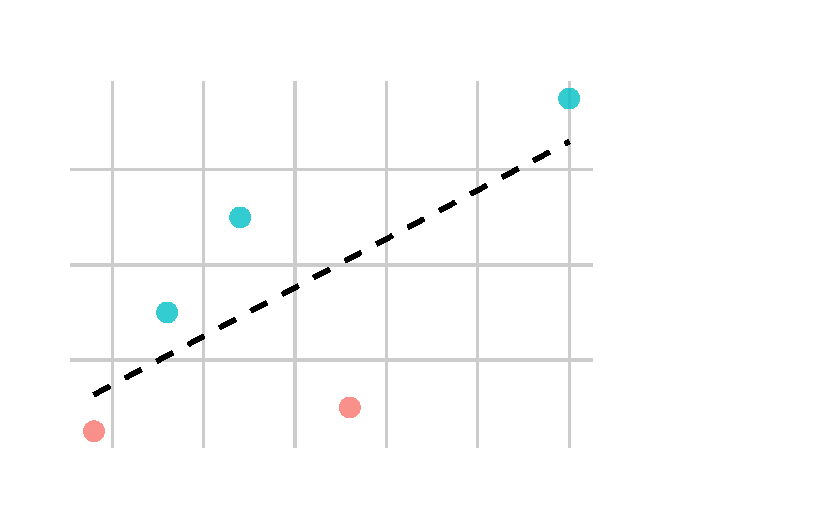
\includegraphics{collaborative_notebook_files/figure-pdf/publication quality figure 1-1.pdf}

}

\caption{Figure 1}

\end{figure}%

\begin{figure}[H]

{\centering 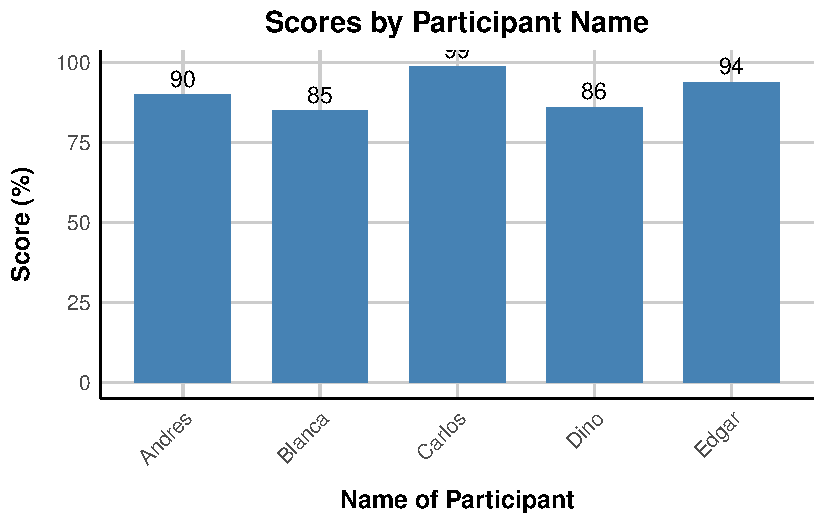
\includegraphics{collaborative_notebook_files/figure-pdf/publication quality figure 2-1.pdf}

}

\caption{Figure 2}

\end{figure}%

\begin{figure}[H]

{\centering 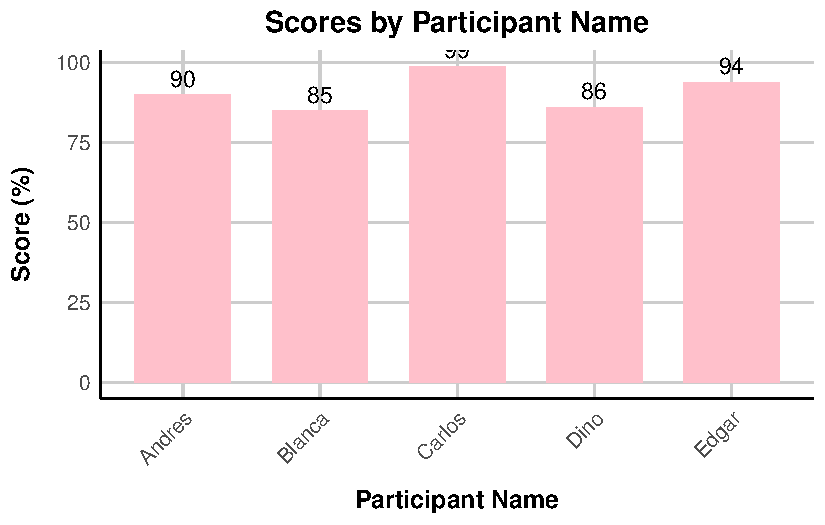
\includegraphics{collaborative_notebook_files/figure-pdf/publication quality figure 3-1.pdf}

}

\caption{Figure 3}

\end{figure}%

\begin{figure}[H]

{\centering 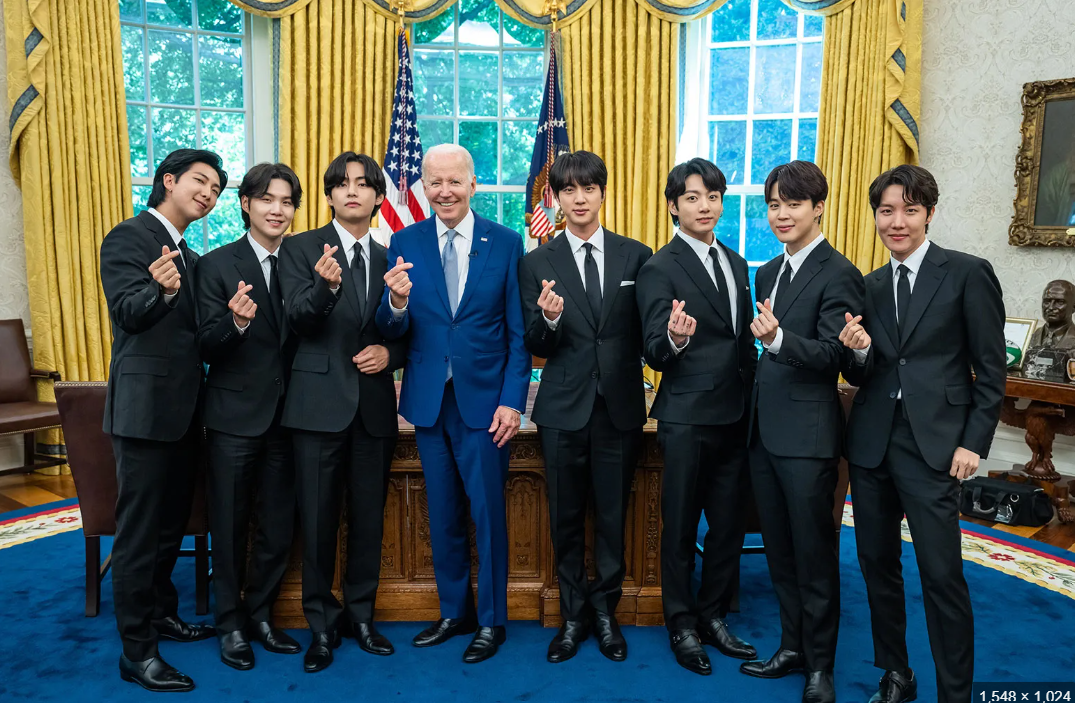
\includegraphics{bts_whitehouse.png}

}

\caption{Image 1}

\end{figure}%

The mean test score is 90.8 .

The highest test score in the data set of given participants is 99 .

The range of participant ages in the data set is from 19 to 45 years
old. The median age in the data set is 27 years old. The youngest person
in the data set who took the exam is Blanca, who is currently 19 years
old.

The data set contains 5 observations, meaning that 5 individuals took
the exam; with the scores ranging from \texttt{rmin(df\$Score)} to
\texttt{rmax(df\$Score)}. The difference between the highest achieved
score and the lowest is 14 percent. In regards to the course sections
enrolled, there were 2 in session A and 3 in session B. In comparing the
two groups, there was an average acore of 85.5 in session A while
session B had an average score of 94.33 percent.

\textbf{Figure 1} shows that there is a relationship between the
participant's age and their test score. Further, the scores themselves
are displayed by their respective participant name in \textbf{Figure 2}.
More information on this data set is given in \textbf{Table 1}.

\section{References}\label{references}

\phantomsection\label{refs}
\begin{CSLReferences}{1}{0}
\bibitem[\citeproctext]{ref-malcolmChangesWithdrawalCraving2018}
Malcolm, Benjamin J., Martin Polanco, and Joseph P. Barsuglia. 2018.
{``Changes in {Withdrawal} and {Craving Scores} in {Participants
Undergoing Opioid Detoxification Utilizing Ibogaine}.''} \emph{Journal
of Psychoactive Drugs} 50 (3): 256--65.
\url{https://doi.org/10.1080/02791072.2018.1447175}.

\end{CSLReferences}




\end{document}
